% !TEX TS-program = pdflatex
% !TEX encoding = UTF-8 Unicode

% This is a simple template for a LaTeX document using the "article" class.
% See "book", "report", "letter" for other types of document.

\documentclass[11pt]{article} % use larger type; default would be 10pt

\usepackage[utf8]{inputenc} % set input encoding (not needed with XeLaTeX)
\usepackage[spanish]{babel}

%%% Examples of Article customizations
% These packages are optional, depending whether you want the features they provide.
% See the LaTeX Companion or other references for full information.

%%% PAGE DIMENSIONS
\usepackage{geometry} % to change the page dimensions
\geometry{a4paper} % or letterpaper (US) or a5paper or....
% \geometry{margin=2in} % for example, change the margins to 2 inches all round
% \geometry{landscape} % set up the page for landscape
%   read geometry.pdf for detailed page layout information

\usepackage{graphicx} % support the \includegraphics command and options
\usepackage[outdir=./]{epstopdf}
% \usepackage[parfill]{parskip} % Activate to begin paragraphs with an empty line rather than an indent
\usepackage{listings}

%%% PACKAGES
\usepackage{booktabs} % for much better looking tables
\usepackage{array} % for better arrays (eg matrices) in maths
\usepackage{paralist} % very flexible & customisable lists (eg. enumerate/itemize, etc.)
\usepackage{verbatim} % adds environment for commenting out blocks of text & for better verbatim
%\usepackage{subfig} % make it possible to include more than one captioned figure/table in a single float
\usepackage{subcaption}
\usepackage{url}
\usepackage{diagbox}
\usepackage{amsmath}
\usepackage{pdfpages}
% These packages are all incorporated in the memoir class to one degree or another...

%%% HEADERS & FOOTERS
\usepackage{fancyhdr} % This should be set AFTER setting up the page geometry
\pagestyle{fancy} % options: empty , plain , fancy
\renewcommand{\headrulewidth}{0pt} % customise the layout...
\lhead{}\chead{}\rhead{}
\lfoot{}\cfoot{\thepage}\rfoot{}

%%% SECTION TITLE APPEARANCE
\usepackage{sectsty}
\allsectionsfont{\sffamily\mdseries\upshape} % (See the fntguide.pdf for font help)
% (This matches ConTeXt defaults)

%%% ToC (table of contents) APPEARANCE
\usepackage[nottoc,notlof,notlot]{tocbibind} % Put the bibliography in the ToC
\usepackage[titles,subfigure]{tocloft} % Alter the style of the Table of Contents
\renewcommand{\cftsecfont}{\rmfamily\mdseries\upshape}
\renewcommand{\cftsecpagefont}{\rmfamily\mdseries\upshape} % No bold!

%%% END Article customizations

%%% The "real" document content comes below...

\title{CLP Lab 2 Report}
\author{Albert Aparicio Isarn\\
	\url{albert.aparicio.isarn@alu-etsetb.upc.edu}
	\and 
	Héctor Esteban\\
	\url{hect.esteban@gmail.com}}
\date{} % Activate to display a given date or no date (if empty),
         % otherwise the current date is printed 

\begin{document}
	
	% ---- MATLAB Code definitions ----- %
	\definecolor{mygreen}{rgb}{0,0.6,0}
	\definecolor{mygray}{rgb}{0.5,0.5,0.5}
	\definecolor{mymauve}{rgb}{0.58,0,0.82}
	
	\lstset{ %
		%backgroundcolor=\color{white},   % choose the background color; you must add \usepackage{color} or \usepackage{xcolor}
		basicstyle=\ttfamily\footnotesize,        % the size of the fonts that are used for the code
		breakatwhitespace=false,         % sets if automatic breaks should only happen at whitespace
		breaklines=true,                 % sets automatic line breaking
		captionpos=b,                    % sets the caption-position to bottom
		commentstyle=\color{mygreen},    % comment style
		deletekeywords={...},            % if you want to delete keywords from the given language
		escapeinside={\%*}{*)},          % if you want to add LaTeX within your code
		extendedchars=true,              % lets you use non-ASCII characters; for 8-bits encodings only, does not work with UTF-8
		%frame=single,	                   % adds a frame around the code
		keepspaces=true,                 % keeps spaces in text, useful for keeping indentation of code (possibly needs columns=flexible)
		keywordstyle=\color{blue},       % keyword style
		language=Matlab,                 % the language of the code
		otherkeywords={*,...},            % if you want to add more keywords to the set
		%numbers=left,                    % where to put the line-numbers; possible values are (none, left, right)
		%numbersep=5pt,                   % how far the line-numbers are from the code
		%numberstyle=\tiny\color{mygray}, % the style that is used for the line-numbers
		rulecolor=\color{black},         % if not set, the frame-color may be changed on line-breaks within not-black text (e.g. comments (green here))
		showspaces=false,                % show spaces everywhere adding particular underscores; it overrides 'showstringspaces'
		showstringspaces=false,          % underline spaces within strings only
		showtabs=false,                  % show tabs within strings adding particular underscores
		stepnumber=2,                    % the step between two line-numbers. If it's 1, each line will be numbered
		stringstyle=\color{mymauve},     % string literal style
		tabsize=2,	                   % sets default tabsize to 2 spaces
		title=\lstname                   % show the filename of files included with \lstinputlisting; also try caption instead of title
	}
	
\maketitle

\section{Clasificación aplicada a la base de datos Phoneme}

En la figura \ref{fig:db:spectrum} se pueden ver los espectros de los fonemas.

\begin{figure}[h]
	\centering
	\includegraphics[width=\textwidth]{../spectrum.eps}
	\caption[]{\small Espectros de los fonemas de la base de datos. En la figura inferior derecha se puede ver el espectro de los promedios de cada fonema.}
	\label{fig:db:spectrum}
\end{figure}

\subsection{Clasificación con 64 características}

En la tabla \ref{tab:db:errors} se muestran las probabilidades de error para los clasificadores Lineal y Quadrático, tanto en entrenamiento (Train) como en Test.

\begin{table}[h]
	\begin{center}
		\begin{tabular}{| l | c | c |}
			\hline
			\diagbox[width=10em]{\textbf{Clasificador}}{\textbf{Fase}} & \textbf{Train} & \textbf{Test} \\
			\hline
			\textbf{Lineal (LC)} & $ 0.073588342440801452 $ & $ 0.08851063829787234 $ \\
			\hline
			\textbf{Cuadrático (QC)} & $ 0.049908925318761385 $ & $ 0.10553191489361702 $ \\
			\hline
		\end{tabular}
		\caption{Probabilidades del error de clasificación de Train y de Test, obtenidas mediante LC y QC usando todas las características.}
		\label{tab:db:errors}
	\end{center}
\end{table}

Las matrices de confusión obtenidas con los clasificadores Lineal y Quadrático en test se encuentran en las ecuaciones \eqref{eq:db:cm:lin} y \eqref{eq:db:cm:quad}, respectivamente.

\begin{equation} \label{eq:db:cm:lin}
\left( \begin{array}{ccccc}
129 & 52 & 0 & 0 & 0 \\
30 & 237 & 0 & 0 & 0 \\
0 & 0 & 190 & 5 & 2 \\
0 & 0 & 2 & 301 & 0 \\
0 & 0 & 0 & 0 & 227 \\ 
\end{array} \right)
\end{equation}

\begin{equation} \label{eq:db:cm:quad}
\left( \begin{array}{ccccc}
122 & 59 & 0 & 0 & 0 \\
49 & 218 & 0 & 0 & 0 \\
0 & 0 & 193 & 3 & 1 \\
0 & 0 & 15 & 284 & 4 \\
0 & 0 & 0 & 0 & 227 \\ 
\end{array} \right)
\end{equation}

La matriz de confusión del clasificador cuadrático en test tiene mayor índice de errores, debida a la tendencia a sobreentrenar que tiene este clasificador.

La matriz del clasificador lineal tiene menos errores en test, cosa que también se refleja en sus probabilidades de error, ya que por sus pocos grados de libertad, debe generalizar más en la clasificación.

\subsection{Clasificación con 2 características}

Para esta sección se han probado dos pares de características: el par $\left(8, 40\right)$ y el par $\left(22, 64\right)$.

Para las componentes 22 y 64, se han elegido componentes que separaran bien todas las componentes a la vez. Sin embargo, el resultado es que los pares de clases 1-2 y 4-5 aparecen mezclados.

Eligiendo las componentes 8 y 40, las clases 4 y 5 se han separado mejor, aunque la pareja 1-2 sigue apareciendo mezclada.

\clearpage

\subsubsection{Par $\left(8, 40\right)$}

Las probabilidades de error obtenidas en este caso se encuentran en la tabla \ref{tab:2c:8_40:prob}.

\begin{table}%[h]
	\begin{center}
		\begin{tabular}{| l | c | c |}
			\hline
			\diagbox[width=10em]{\textbf{Clasificador}}{\textbf{Fase}} & \textbf{Train} & \textbf{Test} \\
			\hline
			\textbf{Lineal (LC)} & $ 0.26156648451730419 $ & $ 0.26978723404255317 $ \\
			\hline
			\textbf{Cuadrático (QC)} & $ 0.253551912568306 $ & $ 0.26638297872340427 $ \\
			\hline
		\end{tabular}
		\caption{Probabilidades del error de clasificación para el par $\left(8, 40\right)$.}
		\label{tab:2c:8_40:prob}
	\end{center}
\end{table}

En la figura \ref{fig:2c:8_40:scatter} se muestra el dibujo del scatter con las fronteras de clasificación.

\begin{figure}[h]
	\centering
	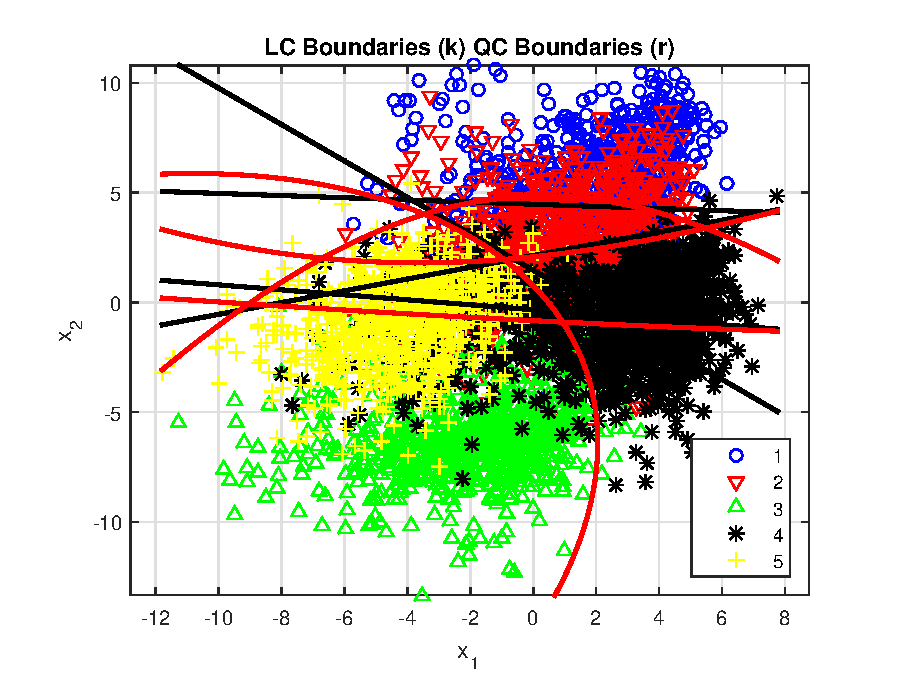
\includegraphics[width=\textwidth]{../2_comp/[8_40].eps}
	\caption[]{\small \emph{Scatter plot} con las fronteras de clasificación obtenidas para la clase ‘aa’ respecto al resto de clases.}
	\label{fig:2c:8_40:scatter}
\end{figure}

\clearpage

\subsubsection{Par $\left(22, 64\right)$}

Las probabilidades de error obtenidas en este caso se encuentran en la tabla \ref{tab:2c:22_64:prob}.

\begin{table}[h]
	\begin{center}
		\begin{tabular}{| l | c | c |}
			\hline
			\diagbox[width=10em]{\textbf{Clasificador}}{\textbf{Fase}} & \textbf{Train} & \textbf{Test} \\
			\hline
			\textbf{Lineal (LC)} & $ 0.28998178506375227 $ & $ 0.28085106382978725 $ \\
			\hline
			\textbf{Cuadrático (QC)} & $ 0.2783242258652095 $ & $ 0.27148936170212767 $ \\
			\hline
		\end{tabular}
		\caption{Probabilidades del error de clasificación para el par $\left(22, 64\right)$.}
		\label{tab:2c:22_64:prob}
	\end{center}
\end{table}

En la figura \ref{fig:2c:22_64:scatter} se muestra el dibujo del scatter con las fronteras de clasificación.

\begin{figure}[h]
	\centering
	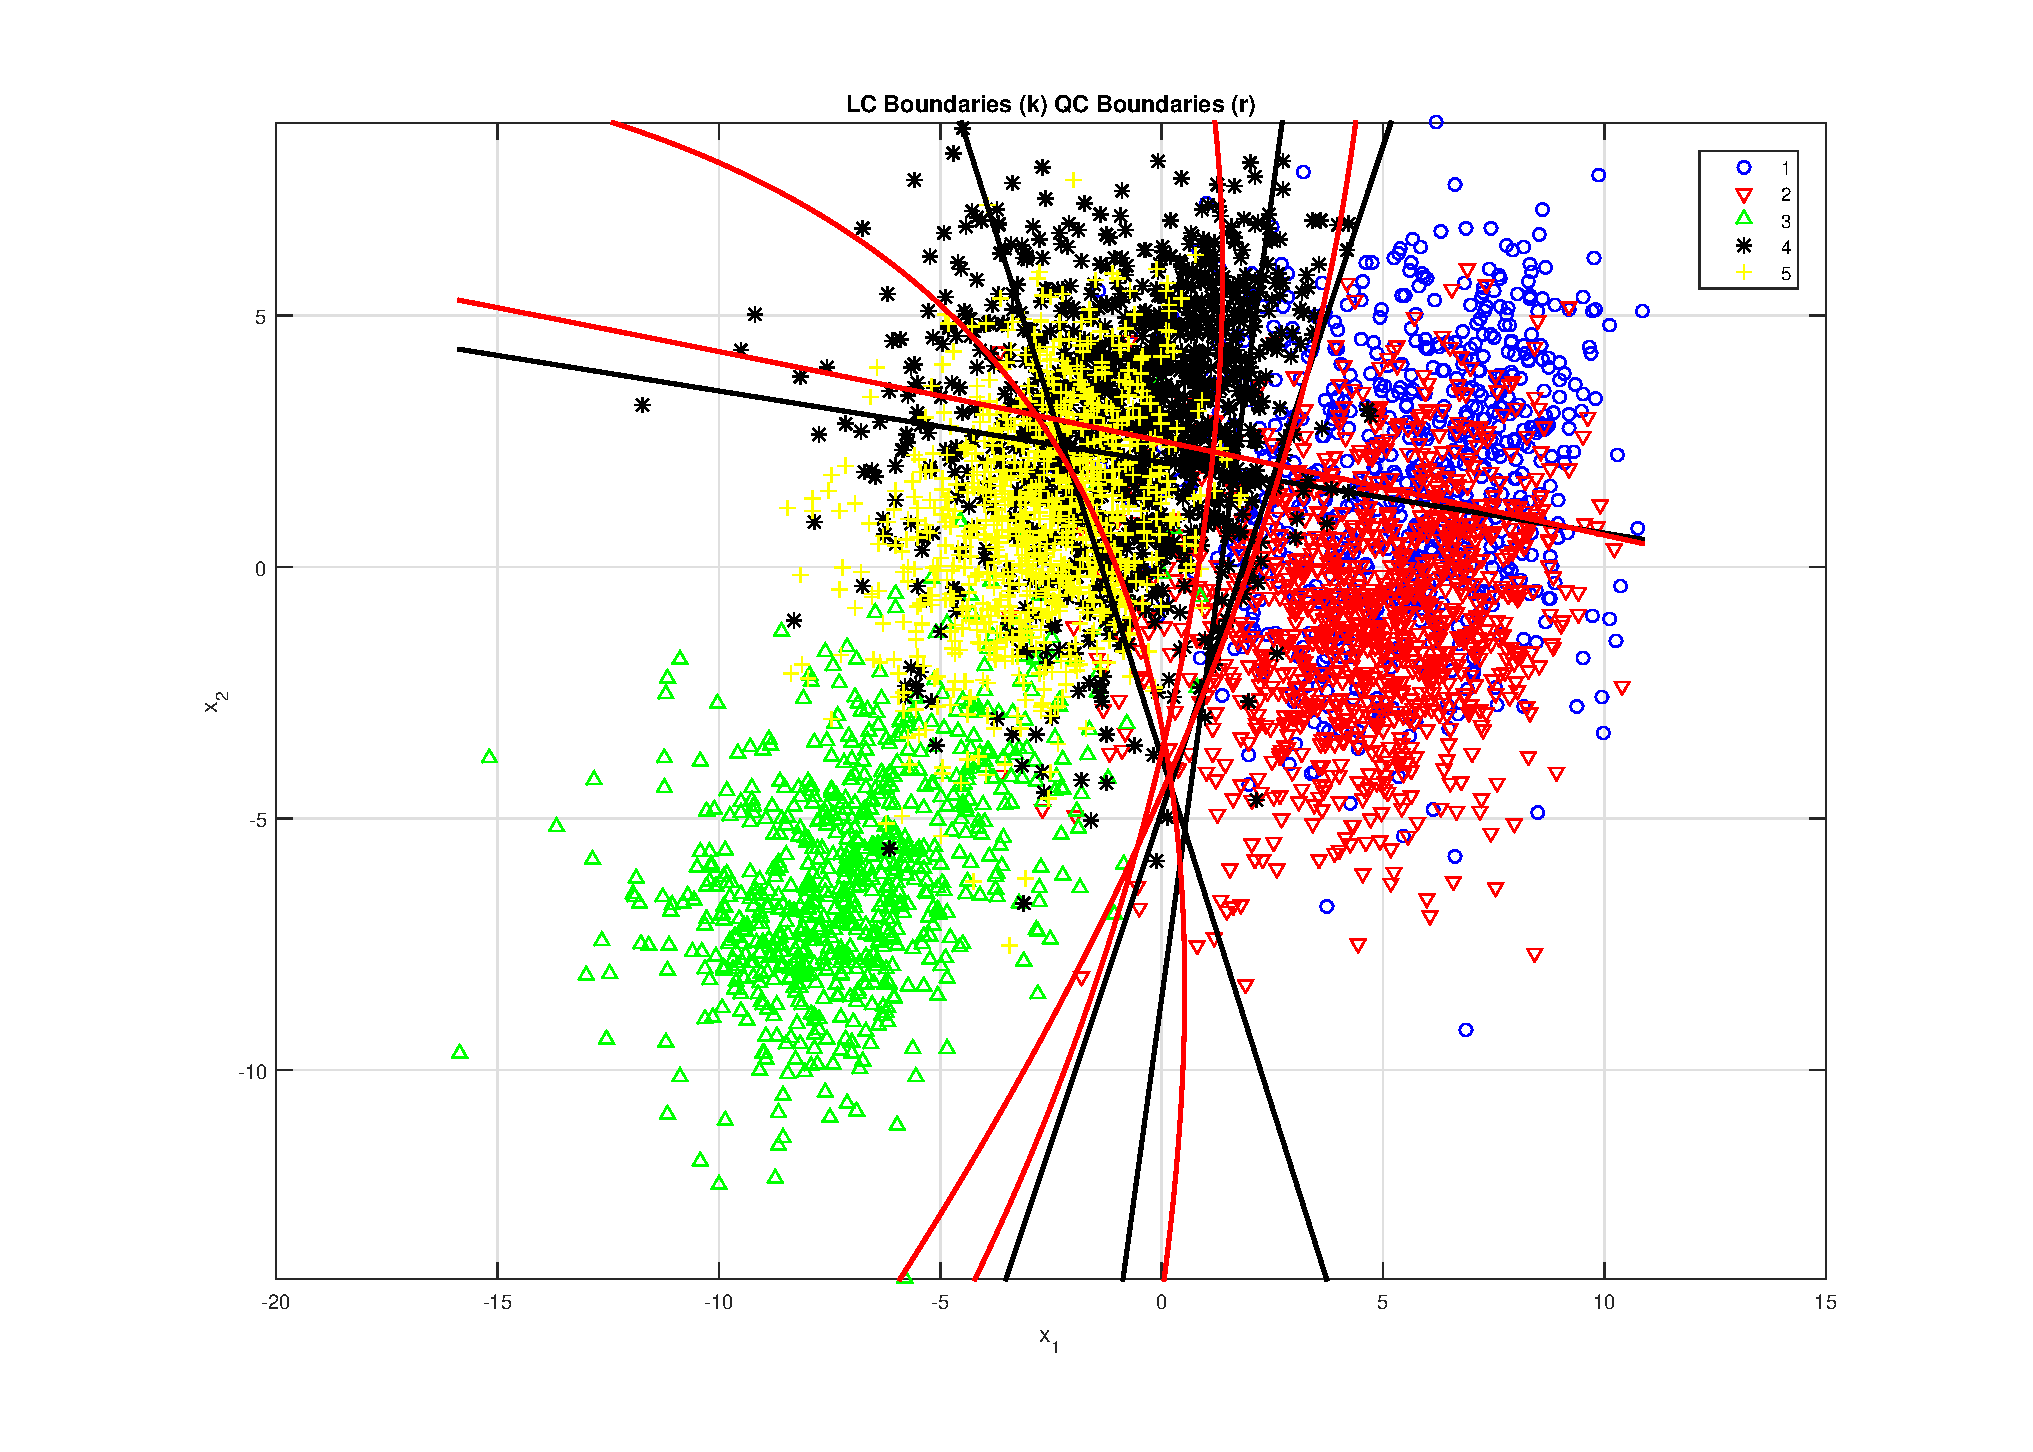
\includegraphics[width=\textwidth]{../2_comp/[22_64].eps}
	\caption[]{\small \emph{Scatter plot} con las fronteras de clasificación obtenidas para la clase ‘aa’ respecto al resto de clases.}
	\label{fig:2c:22_64:scatter}
\end{figure}

\clearpage

\section{Reducción de dimensión mediante PCA}

En las figuras \ref{fig:pca:64} y \ref{fig:pca:256} se muestran las gráficas de los errores de clasificación para 64 y 256 características, respectivamente.

La probabilidad de error del clasificador lineal se queda 'estancada' con menos características que el quadrático, ya que tiene menos grados de libertad y requiere menos características para entrenar el clasificador correctamente.

El código que hace las proyecciones PCA se ha hecho con un bucle paralelo (\texttt{parfor}) de MATLAB, de manera que el tiempo de ejecución se reduce aproximadamente a razón del número de procesadores de que disponga el ordenador.

\begin{figure}[h]
	\centering
	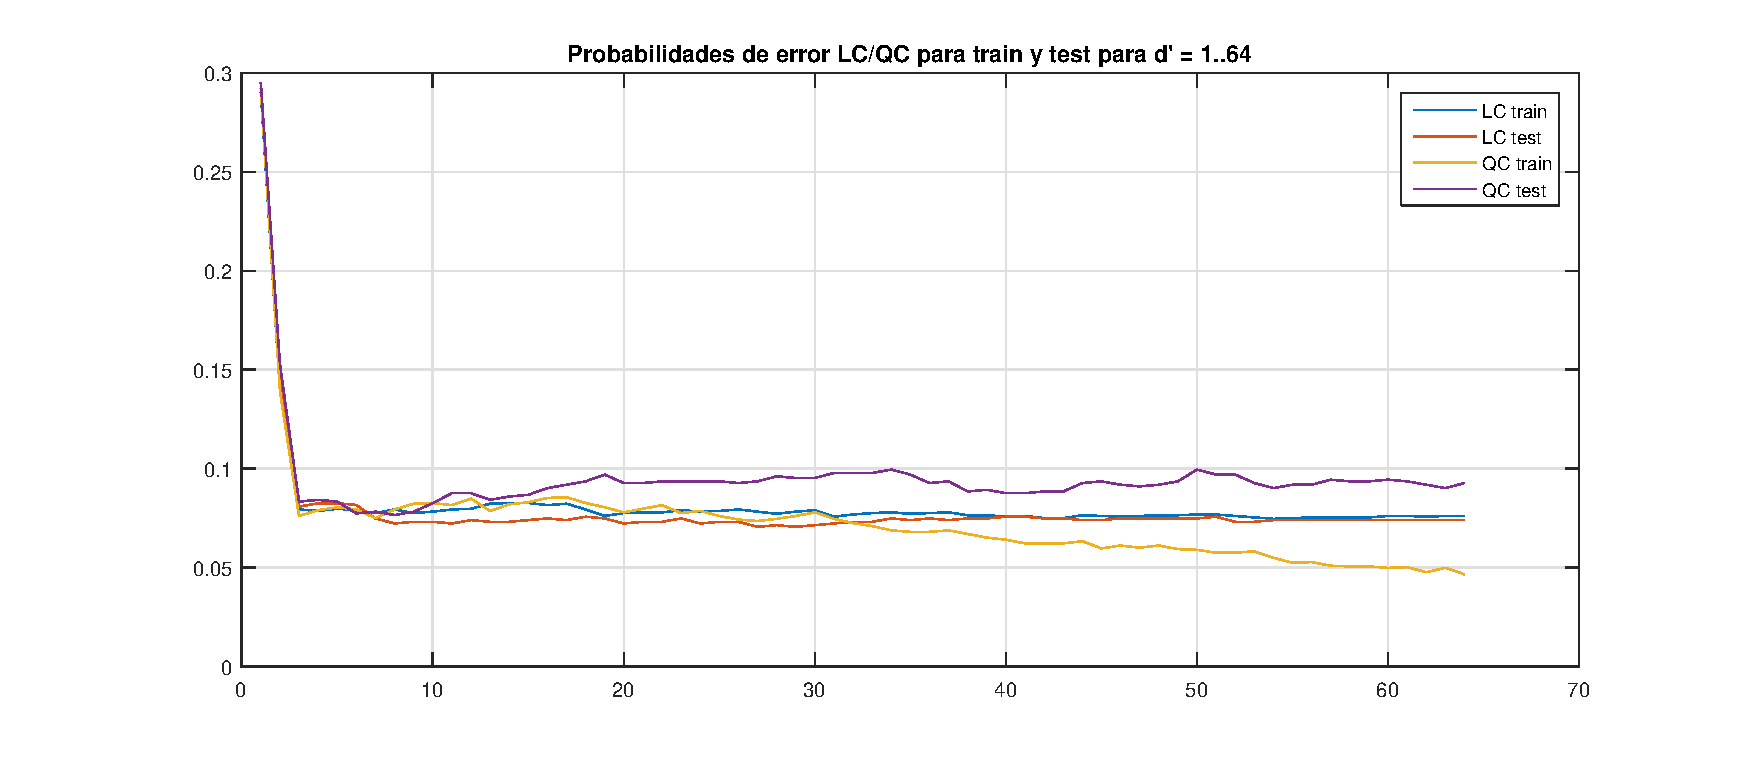
\includegraphics[width=0.9 \textwidth]{../PCA/LC_QC_train_test_64.eps}
	\caption[]{\small Gráfica de probabilidades de error con 64 características.}
	\label{fig:pca:64}
\end{figure}

\begin{figure}[h]
	\centering
	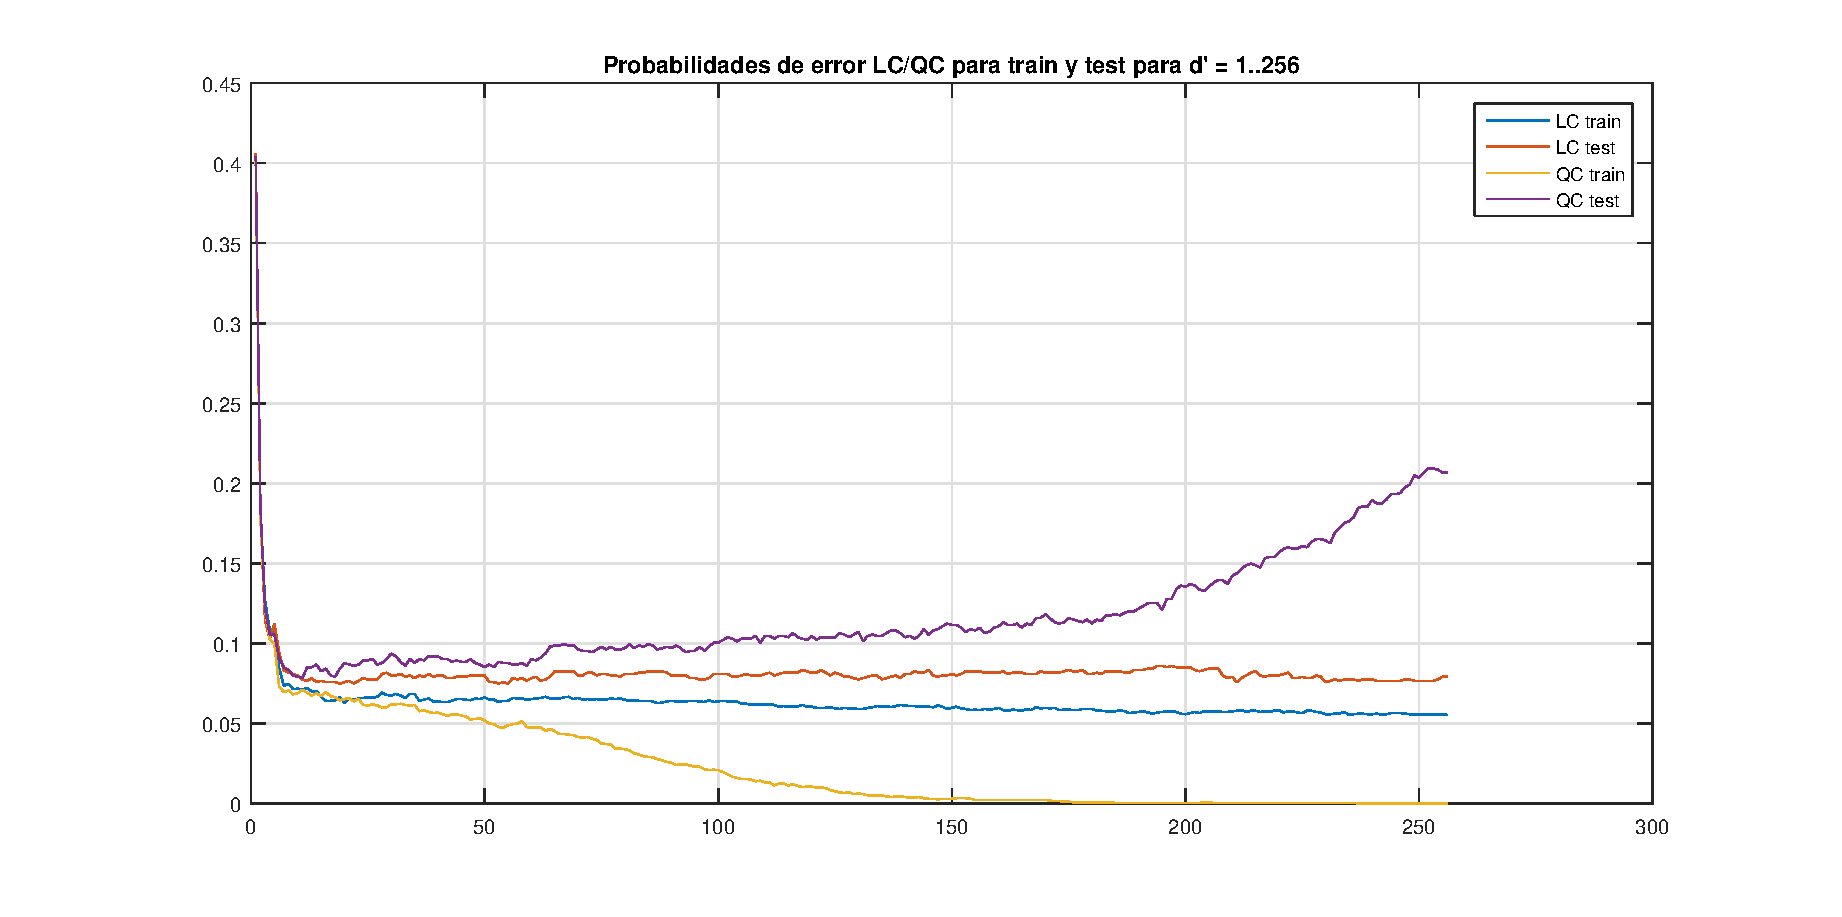
\includegraphics[width=0.9 \textwidth]{../PCA/LC_QC_train_test_256.eps}
	\caption[]{\small Gráfica de probabilidades de error con 256 características.}
	\label{fig:pca:256}
\end{figure}

A continuación se incluye el código de la función \texttt{prac2\_fonemas\_PCA.m}

\clearpage

\lstinputlisting{../prac2_fonemas_PCA.m}

\end{document}
